\documentclass[twoside]{article}

%\usepackage{aistats2019}
% If your paper is accepted, change the options for the package
% aistats2019 as follows:
%
\usepackage[accepted]{aistats2019}
%
% This option will print headings for the title of your paper and
% headings for the authors names, plus a copyright note at the end of
% the first column of the first page.

% If you set papersize explicitly, activate the following three lines:
%\special{papersize = 8.5in, 11in}
%\setlength{\pdfpageheight}{11in}
%\setlength{\pdfpagewidth}{8.5in}

% If you use natbib package, activate the following three lines:
%\usepackage[round]{natbib}
%\renewcommand{\bibname}{References}
%\renewcommand{\bibsection}{\subsubsection*{\bibname}}

% If you use BibTeX in apalike style, activate the following line:
\bibliographystyle{apalike}
\usepackage[round]{natbib} 

\usepackage[utf8]{inputenc} % allow utf-8 input
\usepackage[T1]{fontenc}    % use 8-bit T1 fonts
\usepackage{hyperref}       % hyperlinks
\usepackage{url}            % simple URL typesetting
\usepackage{booktabs}       % professional-quality tables
\usepackage{amsfonts}       % blackboard math symbols
\usepackage{nicefrac}       % compact symbols for 1/2, etc.
\usepackage{microtype}      % microtypography
\usepackage{caption}

%% PGF
\usepackage{tikz,amsmath,amssymb}

\usetikzlibrary{calc,bayesnet,shapes.geometric,arrows,chains,matrix,positioning,scopes,calendar,decorations.markings,decorations.pathreplacing,intersections}

\makeatletter
\tikzset{join/.code=\tikzset{after node path={%
      \ifx\tikzchainprevious\pgfutil@empty\else(\tikzchainprevious)%
      edge[every join]#1(\tikzchaincurrent)\fi}}
}
\tikzset{>=stealth',every on chain/.append style={join},
  every join/.style={->}
}

\newcommand{\inputTikZ}[2]{%  
     \scalebox{#1}{\input{#2}}  
}

\begin{document}

% If your paper is accepted and the title of your paper is very long,
% the style will print as headings an error message. Use the following
% command to supply a shorter title of your paper so that it can be
% used as headings.
%
%\runningtitle{I use this title instead because the last one was very long}

% If your paper is accepted and the number of authors is large, the
% style will print as headings an error message. Use the following
% command to supply a shorter version of the authors names so that
% they can be used as headings (for example, use only the surnames)
%
%\runningauthor{Surname 1, Surname 2, Surname 3, ...., Surname n}

\twocolumn[

\aistatstitle{Learning exponential families}

\aistatsauthor{Anonymous Author(s)}

\aistatsaddress{Affiliation \\ Address \\ email} ]

\begin{abstract}
Recently much attention has been paid to implicit probability models, since they have been used to great success for variational inference, generation of complex data types, and more.  In most all of these settings, the goal has been to find a \emph{particular member} of that model family: optimized parameters index a distribution that is close (via a divergence or classification metric) to a target distribution.  Much less attention, however, has been paid to the problem of \emph{learning a model itself}.   Here we define implicit probability models with specific deep network architectures and optimization procedures for learning intractable exponential family models (\emph{not} a single distribution from those models).  These exponential families, which are central to some of the most fundamental problems in probabilistic inference, are learned accurately, allowing operations like posterior inference to be executed directly and generically by an input choice of natural parameters, rather than performing inference via optimization for each particular realization of a distribution within that model.  
\end{abstract}

\section{Introduction}
Probability models, the fundamental object of Bayesian machine learning, have long challenged researchers with the tradeoff between tractability and expressivity.
Though well understood that a model should be chosen to instantiate a set of assumptions and capture existing domain knowledge \cite{gelman2014bayesian, tenenbaum2006theory, mccullagh2002}, for many years too-simple models were chosen for their practical advantanges (such as conditional conjugacy), which left much to be desired in terms of expressive performance and scalability of these models.  

More recently the pendulum has swung, via a resurgence in models which map a latent random variable $w\sim q_0$ through a member of a highly expressive function family $\mathcal{G} = \left\{g_\theta : \theta \in \Theta\right\}$, the composition resulting in an \emph{implicit probability model} $\mathcal{M} = \left\{ q(g_\theta (w)) : \theta \in \Theta \right\}$ (where $q(\cdot)$ is the pushforward density, i.e. the density induced on the image of the random variable $w$ under the function $g_\theta$).  
Choosing $\mathcal{G}$ to be a parameter-indexed family of neural networks has both a rich history \cite{dayan1995helmholtz,mackay1997density}, and has recently been used to produce exciting results for density estimation \cite{uria2013rnade, rippel2013high, papamakarios2017masked}, generation of complex data \cite{Goodfellow:2014aa}, variational inference \cite{Kingma:2013aa, rezende2014stochastic, titsias2014doubly}, and more.  
A noted advantage of these implicit density network models is that in many cases they make minimal assumptions about the data generative (or posterior inference) process.  
On the other hand, since these models have been chosen to be generic and flexible, they can lack the classic stipulation that a model instantiates existing domain knowledge.  
The downsides of a too-flexible model with finite data (albeit large) -- and the corresponding bias-variance benefit of a restricted model -- are textbook knowledge \cite[\S 7.3]{friedman2001elements}, and work on generalization and compressibility in deep networks suggests that this broad class of function families are indeed quite large, perhaps problematically so \cite{zhou2018compressibility}.  

Is all the flexibility of an implicit density network model $\mathcal{M}$ always necessary?  
Consider the case of variational inference, where a generative model $p(z)p_\beta(X | z)$ (latent $z$, observed data $X$) is stipulated in the classic sense to embody modeling assumptions (hierarchical model, topic model, Bayesian logistic regression, etc.).  
When such a model is intractable, it is increasingly common to deploy an implicit ``recognition network'' model for variational inference \cite{Kingma:2013aa}, which finds a $q_{\theta^*}(z) \in \mathcal{M}$ such that an evidence bound is optimized with respect to the true posterior $p(z|X)$.  
However, note the widely recognized fact \cite{wainwright2008graphical} that many such true posteriors $p(z|X)$ belong to models that can be written as exponential families (albeit intractable, due to the choice of sufficient statistics $t(z)$). %, of the form: $\mathcal{P} = \left\{ \frac{h(z)}{A(\eta)} \exp\left\{ \eta^\top t(z) \right \} : \eta \in H \right\}$.  
Some effort has been made to learn single members of exponential families from mean parameters \cite{loaiza2017maximum}, but we are focused on the natural parameterization and the model itself. 

 Should we be able to learn a tractable approximation to this exponential family model, we would in the very least get the bias-variance benefits of an intelligently restricted model space, and at best would get inference ``for free'' in the sense that we could evaluate approximate posteriors directly without separate optimization for each dataset encountered (a novel form of \emph{amortized inference} \cite{gershman2014amortized,Kingma:2013aa,rezende2014stochastic,stuhlmuller2013learning}).  
 In this paper we aim to learn a restricted model $\mathcal{Q} = \left\{ q(z; \eta: \eta \in H)\right\}$ that will be a strict subset of $\mathcal{M}$ and will closely approximate a target exponential family $\mathcal{P}$.  
 Note the critical difference between this aim and much of the literature that seeks to learn a density $q_{\theta}^* \in \mathcal{M}$ (we explore this distinction in depth both algorithmically and empirically).  
 
To proceed, we must first specify a set of models $\mathbb{Q} = \left\{ \mathcal{Q}_\phi : \phi \in \Phi \right\}$, from which we can learn a single model $\mathcal{Q}_{\phi^*}$, and we must second define a sensible parameter space $H$ of each model.  
To the first, we restrict $\Theta$, the parameter space of $\mathcal{M}$, to be itself the image of a second deep \emph{parameter network} family $\mathcal{F} = \left\{f_\phi : \phi \in \Phi\right\}$, such that $\left\{ f_\phi(\eta) : \eta \in H \right\} \subset \Theta$.
The second part is answered immediately by our choice of target $\mathcal{P}$, an exponential family which by definition has \emph{natural} parameterization $\eta \in H$.  
Thus, appealingly, we know that $H$ is precisely the correct parameter space for $\mathcal{Q}$ (as it defines $\mathcal{P}$), and that the image of $H$ under $f_\phi$ will be of the correct dimensionality within the codomain $\Theta$; approximation error between $\mathcal{Q}$ and $\mathcal{P}$ will be caused by the flexibility and learnability of the parameter network $f_\phi$ and the density network $g_{f_{\phi}(\eta)}$.  

We define this two-network architecture, which we term an \emph{exponential family network} (EFN), and we specify a stochastic optimization procedure over a variant of the typical Kullback-Leibler divergence.  We then demonstrate the ability of EFNs to approximately learn exponential families and the benefits of approximating distributions in such restricted model spaces.  Finally we demonstrate the computational savings afforded by this approach when learning the posterior family of point-process latent intensities, given neural spike responses in primary visual cortex of macaques. 

\section{Exponential family networks}

To define exponential family networks (EFNs), we begin with relevant context for our modeling choice of exponential families (\S2.1).  We then describe the primary network architectural constraint and the background we leverage to satisfy that constraint (\S2.2). We then introduce EFN in detail, including the optimization algorithm used for learning (\S2.3).  The similarities with variational inference are then explored in depth in (\S2.4).

\begin{figure}
 {\centering \inputTikZ{0.55}{figs/fig1/efn1b.tex}  }


  \caption{(A) Graphical model for conditionally iid sampling from an exponential family likelihood.  (B) Hierarchical Dirichlets -- prior $p_0(z)$ (top), three sample conditional Dirichlet datasets $X$ of $N=2, N=20, N=100$ (middle), and three corresponding posteriors that themselves form an exponential family $\mathcal{P}$ (bottom).  (C) Architecture for exponential family network (EFN) -- density network running top to bottom; parameter network running right to left.}
\end{figure}

\subsection{Exponential families as target model $\mathcal{P}$}

We will focus on a fundamental problem setup in probabilistic inference, that of a latent variable $z \in \mathcal{Z}$ with prior belief $p_0(z)$, and where we observe a dataset $X = \left\{x_1,...,x_N\right\} \subset \mathcal{X}$ as conditionally independent draws given $z$.   Updating our belief with data produces the posterior $p(z | X) \propto p_0(z) \prod_{i=1}^N p(x_i | z)$.  This setup is shown as a graphical model in Figure 1A.
% and produces an intractable $p(z|X)$ in all but the rare cases of  known conjugacy or careful historical work (often an inversion, transformation-rejection, or similar custom numerical strategy) that has made these distributions computationally indistinguishable from tractable \cite{Devroye:1986aa}. % It is intriguing then to reflect upon the success that deep networks have offered to function approximation, and ask to what extent we can automate this numerical process, widening the class of effectively tractable distributions.

If we restrict our attention to priors and likelihoods that belong to exponential families $\mathcal{P} = \left\{ \frac{h(\cdot)}{A(\eta)} \exp\left\{ \eta^\top t(\cdot) \right \} : \eta \in H \right\}$, the posterior can be also viewed as an exponential family, albeit almost always intractable \cite{wainwright2008graphical}.  For simplicity we will hereafter suppress the base measure $h(\cdot)$.  Consider:

{\small $$ p_0(z) = \frac{1}{A_0(\alpha)} \exp\left\{ \alpha^\top t_0(z) \right\} $$} 
{\small $$p(x_i|z) = \frac{1}{A(z)} \exp\left\{ \nu(z)^\top t(x_i) \right \},$$}

where $t(\cdot)$ is the sufficient statistic vector, and $\nu(z)$ is the natural parameter of the likelihood in natural form \cite{robert2007bayesian}.   The posterior then has the form:

\begin{equation}
{\small
  p(z | x_1,...,x_N)  \propto  \exp\left\{ \begin{bmatrix} \alpha \\ \sum_i t(x_i) \\ -N \end{bmatrix}^\top\begin{bmatrix} t_0(z) \\ \nu(z) \\ \log A(z) \end{bmatrix} \right\},
  }
\label{eq:1}
\end{equation}

which again is an exponential family, albeit intractable.

To give a concrete example, consider the hierarchical Dirichlet -- a Dirichlet prior $z\sim Dir(\alpha)$ (of dimension $|\mathcal{Z}|$) with conditionally iid Dirichlet draws $x_i | z \sim Dir(\beta z)$, which has been considered historically \cite{mackay1995hierarchical}, and is perhaps most notable for its nonparametric extension \cite{teh2006hdp} (and has relevance for multi-corpus extensions of topic models \cite{blei2003latent, pritchard2000inference}).  
Figure 1B shows the prior for a given $\alpha$ (top), and three examples of datasets that could arise via this generative model (middle).  
A set of basic manipulations shows the hierarchical Dirichlet posterior $p(z|X)$ to be itself an exponential family with natural parameter $\eta = \left[ \alpha -1 , \sum_i \log(x_i) , -N \right]^\top$ and sufficient statistic $t(z) = \left[ \log(z), \beta z , \log(B(\beta z)) \right]^\top$.%\footnote{To be clear this model is an exponential family if $\beta$ is fixed or treated as a latent variable; this fact however will not be important for the development of this paper.}
The corresponding posteriors are shown in Figure 1B (bottom).  

Note importantly that, because the likelihood was chosen to be an exponential family (which is closed under sampling), this form will not change for any choice of $|Z|$-dimensional hiearchical Dirichlet -- any draw from the prior, any $N$, or any particular realization of observed data $X$ (technically the prior need not be exponential family, but we leave it as such for simplicity).  
The exponential family is clearly sufficient for this property, and the Pitman-Koopman Lemma further clarifies that it is also necessary (under reasonable conditions) \cite[\S3.3.3]{robert2007bayesian}.

The critical observation here is that, if we can approximately learn an intractable exponential family (the model itself), then it becomes trivial to perform posterior inference: we simply use the dataset to index into the natural parameter $\eta$ of the intractable family, and the posterior distribution is produced.  This is the goal of EFNs.

\subsection{Density networks as generic approximating family $\mathcal{M}$}

Implicit probability models, which we will use for our approximating model family $\mathcal{M}$, can be defined by any base random variable $w\sim p_0$ mapped through any measurable, parameter-indexed function family  $\mathcal{G} = \left\{g_\theta: \theta \in \Theta\right\}$; we denote the induced density on $z=g_\theta(w)$ as $q_\theta(z)$.   
Though trivial to sample from $q_\theta(z)$ for any choice of family $\mathcal{G}$, we here additionally require that we be able to explicitly calculate $q_\theta(z)$.  
This goal can be readily achieved by designing $\mathcal{G}$ to contain only bijective functions, ideally with a Jacobian form that is convenient to compute. %such that $q_\theta(z) = \frac{1}{|J_\theta(z)|} q_0\left(g_\theta^{-1}(z)\right)$ is convenient to compute.   
Designing that bijective $\mathcal{G}$ as a deep neural network family, as we do here, is a well-established idea that has recently seen many variants and applications \cite{mackay1997density, baird2005one, tabak2010density, rippel2013high, uria2013rnade, rezende2015variational, dinh2016density, papamakarios2017masked, jacobsen2018revnet}.  Specifically, let $z = g_\theta(w) = g_L \circ ... \circ g_1(w)$ for bijective vector-valued functions $g_\ell$ (surpressing $\theta$), and denote $J^\ell_\theta(z)$ as the Jacobian of the function $g_\ell$ at the layer activation corresponding to $z$.  Then we have:
%
{\small $$q_\theta(z) = q_0\left( g_1^{-1} \circ ... \circ g_L^{-1}(z) \right) \prod_{\ell=1}^L \frac{1}{| J^\ell_\theta(z) |}.$$}
%
The specific form of the layers $g_\ell$ can be chosen based on empirical considerations; we clarify our choice in \S3.  For the remainder (and to avoid confusion when we introduce a second network) we call this deep bijective neural architecture the \emph{density network}; this network is shown vertically oriented (flowing from $w$ down to $z$) in Figure 1C.

This density network induces the model $\mathcal{M} = \left\{ q(g_\theta \circ w) : \theta \in \Theta \right\}$, which previous work has searched to find a single optimized distribution (such as a posterior or data generative density), on the assumption and subsequent empirical evidence that the target exponential family member is close to (or approximately belongs to) $\mathcal{M}$.   We make the same assumption for the exponential family itself and seek to intelligently restrict $\mathcal{M}$ in order to learn the exponential family.  

\subsubsection{Exponential family networks as approximating model $\mathcal{Q}$}

Having introduced our target model $\mathcal{P}$, an exponential family with natural parameters $\eta \in H$, and the density network family $\mathcal{M}$, we now seek to learn $\mathcal{Q} \approx \mathcal{P}$, where $\mathcal{Q} \subset \mathcal{M}$.  
To do so we will parameterize $\theta$, the parameters of the density network, as the image of a second \emph{parameter network} family $\mathcal{F} = \left\{ f_\phi : H \rightarrow \Theta, \phi \in \Phi\right\}$.   
This network is shown flowing from right to left in Figure 1C.  
Using a second meta-network to aid or restrict network learning has been used in a variety of settings; a few examples include parameterizing the optimization algorithm in the so-called ``learning to learn'' setting \cite{andrychowicz2016learning}, and a more closely related work that used a second network to condition on observations for local latent variational inference \cite{rezende2015variational}, a connection which we explore closely in the following section.

Any choice of parameter network parameters $\phi$ induces a $|H|$-dimensional submanifold (the image $f_\phi(H)$) of the density network parameter space $\Theta$, and as such defines a restricted model $\mathcal{Q}_\phi = \left\{ q_{f_{\phi}}(z; \eta): \eta \in H\right\} \subset \mathcal{M}$; by our choice of $H$ as the natural parameter space of the exponential family target $\mathcal{P}$, this model restriction is at least of the correct dimensionality.
Our goal then is to search over the implied set of models $\mathbb{Q} = \left\{ \mathcal{Q}_\phi : \phi \in \Phi \right\}$ to find an optimal $\phi^*$ such that $\mathcal{Q}_{\phi^*} \approx \mathcal{P}$. 

Given the connections between the exponential family and Shannon entropy, we will measure the error between $\mathcal{Q}_{\phi}$ and $\mathcal{P}$ with Kullback-Leibler divergence.  Consider for the moment a fixed choice of natural parameter $\eta$; we seek to minimize, over $\phi$:

{\small 
\begin{multline*} D\left( q_\phi(z;\eta) || p(z;\eta) \right) \propto \mathbb{E}_{q_\phi} \Bigg( \log q_\phi(z;\eta) - \eta^\top t(z) \Bigg) \\ = \mathbb{E}_{q_\phi} \left( q_0\left( g_\theta^{-1}(z)\right) + \sum_{\ell=1}^L  \log | J^\ell_\theta(z) | - \eta^\top t(z) \right),
\end{multline*} }

where again we note that $\theta = f_\phi(\eta)$, and thus for a fixed eta, this objective depends only on $\phi$.  Indeed, the target $\eta^\top t(z)$ is linear in $\eta$ (an obvious restatement of the log-linear exponential family form), giving us some hope that we may be able to learn this model.  As a side note, this objective can also produce approximations of the log partition (as the intercept term implied by this linear target), which we have found to be reasonably accurate, though nuanced schemes are likely appropriate \cite{papamakarios2015distilling}; we do not explore that further here.

Of course we seek to approximate not just a single target exponential family member ($p(z;\eta)$ for a fixed $\eta$), but rather the entire model $\mathcal{P} = \left\{p(z;\eta): \eta \in H\right\}$.   For optimization we thus need to introduce a distribution $p(\eta)$ (for sampling), leading to the objective: 

{\small 
\begin{multline*}
arg\!\min_{\!\!\!\!\!\!\!\!\!\!\!\phi} \mathbb{E}_{p(\eta)} \left( D\left( q_\phi(z;\eta) || p(z;\eta) \right)\right) \\ =  \arg\!\min_{\!\!\!\!\!\!\!\!\!\!\!\phi}  D\left( q_\phi(z;\eta)p(\eta) || p(z;\eta)p(\eta) \right). 
\end{multline*} }

Unbiased estimates of this objective are immediate: $q_\phi(z;\eta)$ is sampled by computing the density network parameters $\theta = f_\phi(\eta)$ (using the parameter network), sampling the latent $w \sim p_0(w)$, and running that $w$ through the density network; $p(\eta)$ is user defined and thus trivial to sample.  Stochastic optimization can then be carried out on the estimator:   


{\small 
\begin{equation}
\begin{split}
 \mathbb{L}(\phi) = \frac{1}{K}\frac{1}{M}\sum_{k=1}^K & \sum_{m=1}^M \bigg( q_0\left( g_{\theta^k}^{-1}\left(z^m\right)\right) \\ & + \sum_{\ell=1}^L  \log | J^\ell_{\theta^k}\left(z^m\right) | - \eta_k^\top t\left(z^m\right) \bigg),
\end{split}
\label{eq:obj}
\end{equation} }

where $\theta^k = f_\phi\left(\eta_k\right)$.  Successful optimization over $\phi$ should thus result in $\mathcal{Q}_{\phi^*} \in \mathbb{Q}$ that accurately approximates the target exponential family; that is, $\mathcal{Q} \approx \mathcal{P}$.  We call this two-network architecture and optimization an exponential family network (EFN).   What remains for empirical implementation is to make particular choices of hyperparameters, network layers, and optimization algorithm, which we specify in \S3 below.

\section{Relation to variational inference}

A tremendous amount of work in recent years has gone into variational inference (VI), and its similarity to EFN warrants careful attention. 
In the following, we aim to carefully (and somewhat pedantically) dissect this question.  
As such, though EFN can address any target exponential familiy, to bring us closest to VI let us here restrict the EFN target model $\mathcal{P}$ to be a family of posterior distributions.  
%First, we consider the differences in the problem being solved by VI and EFN.  Second, we consider the key mechanical differences that offer some insight into VI. Third, we highlight recent VI work that has particular proximity to EFN.  

The typical role of variational inference is to infer an approximate posterior $q_\phi(z) \approx p(z |X)$.  
In this setting, the difference with EFN is stark, in so much as VI learns this single posterior approximation, whereas the main goal of the EFN is to approximate the model $\mathcal{P} = p_\eta(z|X): \eta \in H$: to learn the family of distributions.  
More recently, much focus has gone into the particular instance of VI for local variables $z_i$, for example $\prod_{i=1}^N p(z_i)p(x_i | z_i)$ (such as a variational autoencoder \cite{Kingma:2013aa}) or  $p(u)\prod_{i=1}^N p(z_i|u)p(x_i | z_i)$ (latent Dirichlet allocation being a canonical example \cite{blei2003latent,blei2017variational}), the result of which is often an amortized inference/recognition network that produces a local variational distribution $q_{\phi^*}(z_i | x_i)$.  
This local variational distribution is typically parameterized explicitly: the inference network $\mu_\phi(x_i)$ induces a local parametric distribution, often a Gaussian $q(z_i | x_i) \sim \mathcal{N}\left(z_i; \mu_\phi(x_i)\right)$ \cite[for example]{Kingma:2013aa}.  Viewed this way, local-latent-variable VI methods induce a model $\left\{  q_{\phi^*}(z_i | x_i) : x_i \in X \right\}$ for a finite dataset $X$.   In that sense, EFN and VI are similar `model learning' approaches.
Even more closely, as part of a long-standing desire to add structure to VI beyond mean-field (classically \cite{saul1996exploiting, barber1999tractable}; more recently \cite{hoffman2015stochastic,tran2015copula}, to name but a few), in several cases a inference network has been used to parameterize a deep implicit model (in a two-network inference architecture, to say nothing of whether or not the generative model itself is a deep implicit model); closest to the EFN architecture is \cite{rezende2015variational} (cf. Figure 2 of \cite{rezende2015variational} with Figure 1C here).   Thus EFN (when used for posterior families) can be seen as a close generalization of VI.   

However, even accepting this VI-as-a-model view, the difference between the finite dataset $X$ and the natural parameter space $H$ persists when viewed at a mechanical level; well-known are the overfitting/generalization issues associated with a finite dataset compared with access to a distribution $p(\eta)$.    Thus one goal of EFN is to allow the model $\mathcal{Q}_{\phi^*} \approx \mathcal{P}$ to be learned in the absence of a finite dataset, such that inference on that dataset can then be executed without concerns of overfitting to that set (and of course without having to run a VI optimization for every new dataset).   Perhaps more importantly, the ``model'' implied by VI is parameterized by $x_i$, and indeed the inference network takes $x_i$ as input.  The EFN on the other hand is considerably more general:  as Equation \ref{eq:1} shows, the posterior includes the natural parameters of the prior, allowing the EFN architecture to learn across a more general setting that VI can not (since any VI inference network is only parameterized by data).  One final difference made clear by Equation \ref{eq:1} is that the observations are given to the EFN \emph{in natural form} (that is, $t(x_i)$, not $x_i$) \cite{robert2007bayesian}.  This choice is a novel insight: by exploiting the known sufficiency of $t(x_i)$ in the target model $\mathcal{P}$, some difference in performance for VI may be observed.  We explore this empirically in the following section.

Accordingly, while EFN and VI do at a high level bear multiple similarities, the differences are both material and provoke interesting speculation about means to improve both VI and EFN.


\section{Results}

We perform a number of experiments to investigate the performance of EFN.  First, we test the ability of EFN to approximate the target model $\mathcal{P}$ when this model is a known, tractable exponential family: this choice provides a simple ground truth and calibrates us to expected performance vs alternatives.    The main advantage of learning an EFN is to make tractable a previously intractable exponential family (at least approximately).  This confers major benefits in terms of test-time: for example, rather than optimization needing to be run for variational inference with each particular dataset realized from a model class, EFN will allow immediate lookup.  This benefit is orders of magnitude and is not instructive to view, so here we focus our analyses on the costs of doing so: what approximation loss is suffered when learning a whole family vs a single distribution.  

To compare model approximations by EFNs to standard methodology, we alternatively train density networks to approximate members of the target model family.  It seems unnecessary to carry around an entire parameter network $f_\phi(\eta)$ if that $\eta$ will not change; thus we dispose of the parameter network and train the density network directly over $\theta$ (again with a deterministic choice of a single $\eta$).  When the distribution being approximated is a posterior, this procedure is variational inference.  We refer to this alternative as NF for normalizing flow.


We also must make some particular architectural choices for these experiments.  
We considered a variety of density network architectures; in all the results we use the planar flow layer introduced in \cite{rezende2015variational}.  
The parameter network was given $\tanh$ nonlinearities. 
In many of the results below we will analyze EFNs across a range of model dimensionality $D$ (that is, $z \in \mathcal{Z} \subseteq \mathbb{R}^D$).    In all cases then we have also $D$ planar flow layers in the density network, with $2D+1$ density network parameters per layer.  In analyses where $D$ was less than 20, 20 planar flows were used.  The number of layers in the parameter network scaled as the square root of $D$, with a minimum of 4 layers, and the number of units per layer scaled linearly from the input to the number of density network parameters. Models were trained using the ADAM optimizer algorithm, with learning rates ranging from $10^{-3}$ to $10^{-5}$.  Optimizations ran for at least 50,000 iterations, and completed once there was a subthreshold increase in ELBO. These choices were made so that model performance saturated, and were held constant within comparative analyses.
All code was implemented in tensorflow, and will be available at {\tt https://github.com/anonymous/}.







\subsection{Tractable exponential families}

Here we study the multivariate Gaussian and Dirichlet families, which offer a known ground truth and intuition about the range of performance that EFN -- learning a model – has with respect to its single-distribution counterpart NF. 
%
\begin{figure}
  \centering
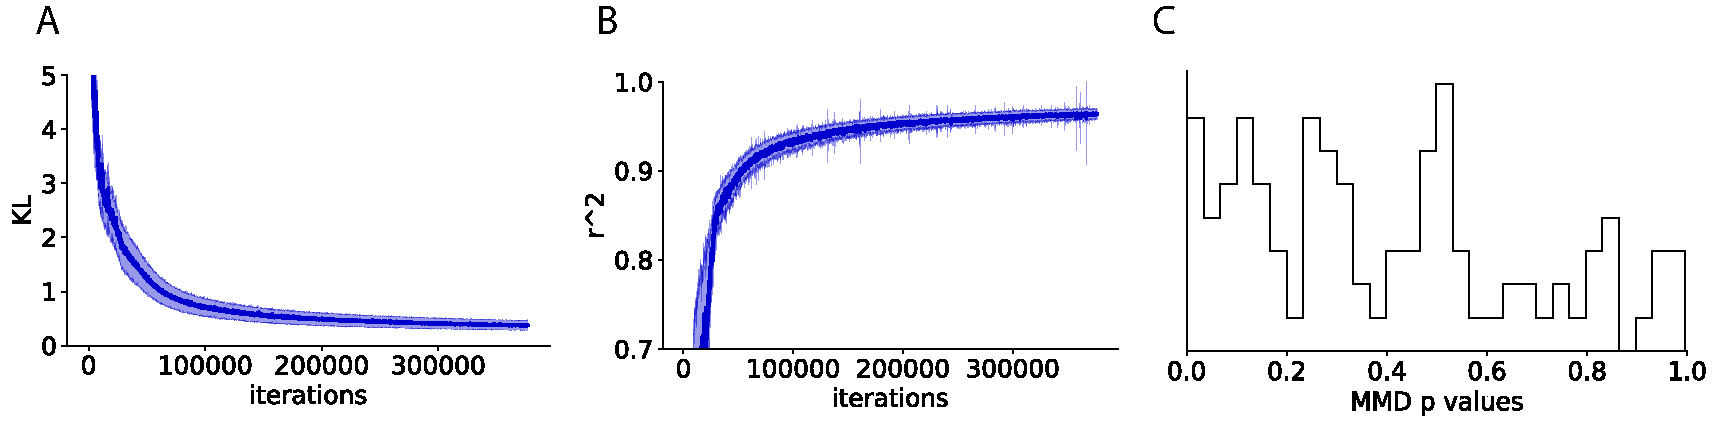
\includegraphics[width=1.0\linewidth]{figs/fig2/fig2.pdf}
  \caption{50-dimensional Dirichlet exponential family network.  (A) Distribution of $r^2$ between log density of EFN samples and ground truth across choices of $\eta$ throughout optimization.  (B) Distribution of KL divergence throughout optimization.  (C) Distribution of maximum mean discrepancy p-values between EFN samples and ground truth after optimization.}
\end{figure}
%
First, to validate the basic EFN approach, we train the $D=50$-dimensional Dirichlet family.  We chose $p(\eta)$, the prior on the $\alpha$ parameter vector of the Dirichlet, as $\alpha_i \sim U\left[.5, 5.0\right]$. The number of $\eta$ samples $K$ at each iteration was $100$, and the minibatch size in $z$ was $M=1000$.   Figure 2 shows a high accuracy fit to this Dirichlet model: Figures 2A and 2B shows rapid convergence to high $r^2$ and low Kullback-Leibler divergence.  $r^2$ is a convenient metric in so much as we are here doing distribution regression, so we calculate the coefficient of determination between the model predictions $\log (q_\phi(z_i; \eta_k))$ and their known targets $\eta_k^\top t(z_i)$.  We can then perform a standard MMD-based kernel two-sample test \cite{gretton2012kernel} between distributions chosen from $\mathcal{P}$ and $\mathcal{Q}_{\phi^*}$: the unstructured distribution of $p$ values clarifies that the EFN model $\mathcal{Q}_{\phi^*}$  is not statistically significantly different than the true target Dirichlet family $\mathcal{P}$ (using a test with 100 samples).

Second, in Figure 3 we consider how this performance scales across dimensionality.  Consider EFN vs NF, where again the only difference is that EFN attempts to learn the entire model (as in $\eta \in H$), whereas NF chooses a single $\eta$ and thus learns a single distribution optimizing the density network parameters $\theta$ directly.  One might expect a noticeable deficit in distributional approximation by EFNs, since they are generalizing the expressivity of the density network across $p(\eta)$.  Accordingly, this deficit is apparent when modeling the multivariate normal family (Fig. 3A).  In low dimensions, we have nearly exact model approximation by EFNs (blue) and distributional approximations by NFs (red).  The distributions learned by NFs were drawn from the same $\eta$ prior as the EFN was trained.  However, as dimensionality increases EFN distributional approximations become significantly worse than the nearly perfect approximations learned by NFs.  The $\eta$ prior of the multivariate normal was specified as an isotropic normal on the mean parameter $\mu_i \sim \mathcal{N}(0, 0.1)$, and an inverse-Wishart distribution on the covariance $\Sigma \sim IW(n, \Psi)$ with degrees of freedom $n=5$ and $\Psi = nD I$.

%
 \begin{figure}
  \centering
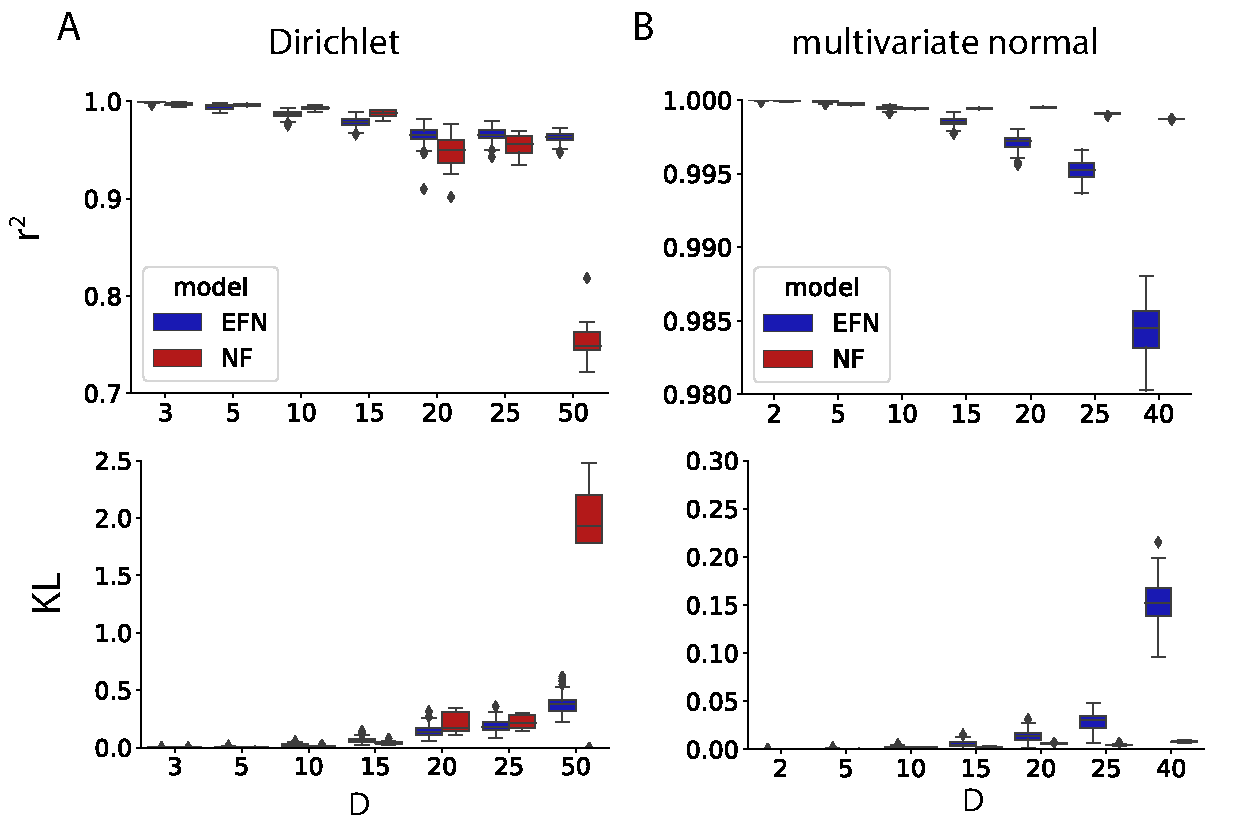
\includegraphics[width=1.0\linewidth]{figs/fig3/fig3.pdf}
  \caption{Scaling exponential family networks: $D$ denotes the dimensionality of the family being learned, and comparisons are between EFN and its $K=1$ alternatives NF1 and EFN1 (see text).  (A) Dirichlet family (B) Gaussian family  (C) Inverse-Wishart family.}
\end{figure}
%

However, learning the model with EFN does not necessarily harm the distributional approximation relative to NF.  In fact, conventional wisdom suggests that learning in a restricted model space often has regulatory benefits.  This is not necessarily the classical bias-variance tradeoff one observes with maximum likelihood or posterior inference in models with varying degrees of restriction.  Here, the expansiveness of the $\eta$ prior determines the necessary degree of generalization of the EFN assigning a weight in the objective to the approximation loss of each distribution.  By requiring the parameter network to learn generalizations of the density network across the $\eta$ prior,  local minima may be avoided that NFs would otherwise be susceptible to.  This is in fact what we see when modeling the Dirichlet distribution (Fig. 3B).  In low dimensions, NF performs better than EFN, but from 20 dimensions and greater, the restricted model space of the EFN confers superior optimization convergence relative to NF, which is more susceptible to local minima.


\subsection{Look-up inference in an intractable exponential family}

Of course the main interest of an EFN is to learn intractable exponential families.  The normal family is the ubiquitous prior for real valued parameters, but it does not match well with the nonnegativity requirements of the intensity measure required of certain distributions, most notably the Poisson.  Log Gaussian Cox Processes have been used numerous times in machine learning, and all have required attention to approximate inference in this fundamentally nonconjugate model; furthermore, very many of these examples have been used to analyze the latent firing intensity of neural spike train data \cite{cunningham2008fast,cunningham2008inferring,adams2009tractable,gao2016linear}.
Here, we trained an EFN to learn the 20-dimensional log-normal Poisson posterior inference family.  This gives us a model of the posterior distribution for a given prior covariance, and some chosen spiking responses.  We demonstrate the utility of such a model on responses of neurons in primary visual cortex of anesthetized macaques to drift grating stimuli at 6.25 Hz \cite{smith2008spatial}.  We can compare the posterior distribution learned with variational inference (red) for a given neuron’s response, to the posterior distribution we get with immediate look-up after training an EFN (blue) (Fig. 4A-B).  These posteriors are very similar, and neither fits the data better than the other.  

Training an EFN understandably takes more time than an NF (Fig. 4C), but once the EFN is trained we have immediate posterior inference lookup.  If we have a target level of approximation (ELBO target) we can determine when it is faster to get posterior inference on a number of datasets by training an EFN and then using the immediate lookup feature or by running variational inference independently for each distribution.  By computing the amount of computational time it takes to reach the ELBO target on average for both EFN and NF, and then counting how many datasets it would take to learn with NF before eclipsing the training time for the EFN.  This results in a decision boundary (Fig. 4D), where an EFN is more computationally efficient for running posterior inference, and we have infinite computational savings for each additional dataset.


\begin{figure}
\centering
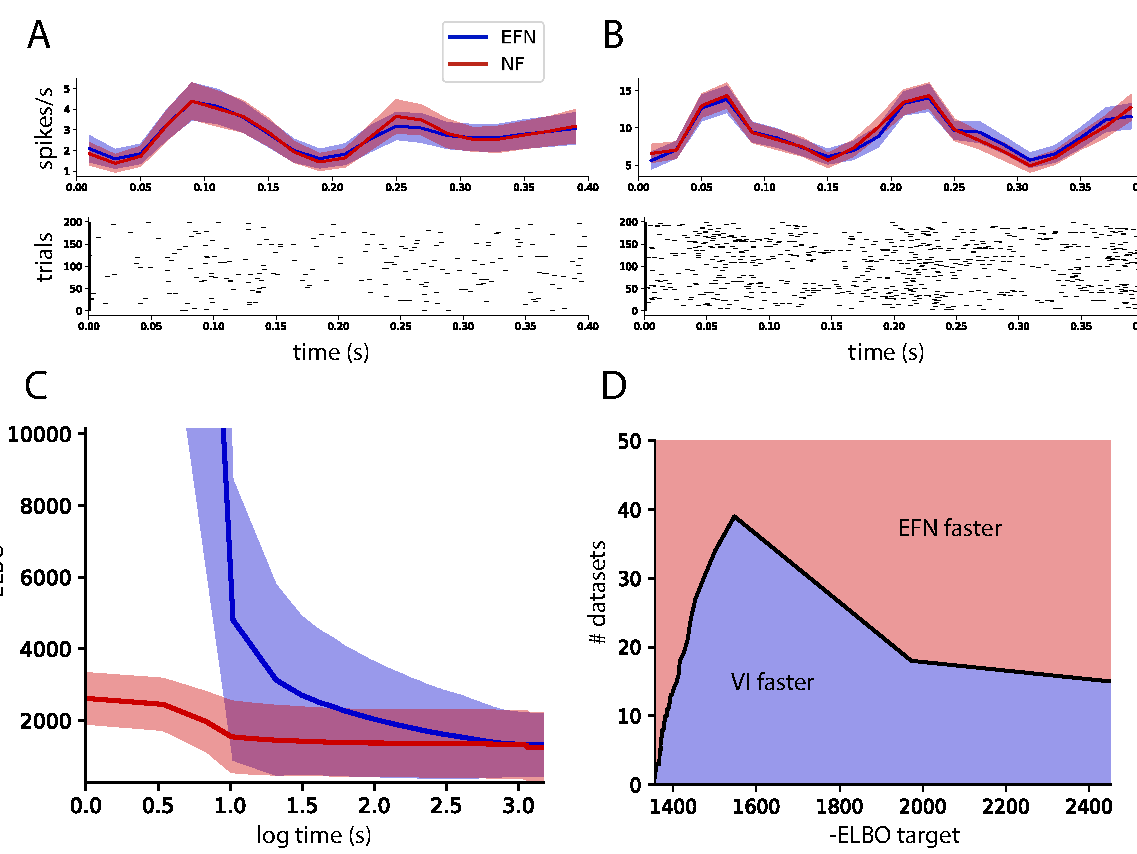
\includegraphics[width=1.0\linewidth]{figs/fig4/fig4.png}
\captionof{figure}{Dirichlet families.  See text.}
\label{fig:test1}
\end{figure}

\section{Conclusion}

We have approached the problem of learning an exponential family, using a deep density network as an implicit probability model, the parameters of which are the image of the natural parameters of the target exponential family under another deep neural network.  
We demonstrated high quality empirical performance across a range of dimensionalities, making a number of previously intractable distributions, including posterior distributions, approximately tractable.

\subsubsection*{Acknowledgements}

Acknowledge the homies.

\subsubsection*{References}

\bibliography{BittnerAIStats2019}
\end{document}
